\graphicspath{{5regression/asy/}}

\section{Regression Models}

We've studied several types of function and seen how to spot whether a given data set might suit a particular model. To get further with this analysis, we need a method for comparing how bad a particular model is for given data.

\subsection{Best-fitting Lines and Linear Regression}\label{sec:reg1}

We start with an example of some data which appears reasonably linear.

\begin{example}{}{reg1}
	At $t$ p.m., a trail-runner's GPS locator says that they've travelled $y$ miles along a trail;\par
	\begin{minipage}[t]{0.64\linewidth}\vspace{-11pt}
		\[
			\begin{array}{c|ccccc}
			t_i&1&2&3&5\\\hline
			y_i&4&8&10&21
			%y&3&7&11&15&19
			\end{array}
		\]
		We'd like a simple model for how far the runner has travelled as a function of $t$. We might use this to predict where they would be at a given time; say at 6\,p.m., or at 2\,p.m.{} if they were to attempt the trail on another day.
	\end{minipage}
	\hfill
	\begin{minipage}[t]{0.35\linewidth}\vspace{-3pt}
		\flushright\includegraphics{reg-line}
	\end{minipage}
	\smallbreak
	By plotting the points, the relationship looks to be approximately\footnotemark{} \textcolor{blue}{linear}: $y\approx mt+c$. What is the \emph{best} choice of line, and how should we find the coefficients $m,c$?\medbreak

	What might be good criteria for choosing our line? What should we mean by \emph{best}? Plainly, we want the points to be close to the line, but measured how? What use do we want to make of the approximating line?\smallbreak

	Here are three candidate lines plotted with the data set: of the choices, which seems best and why?
	\begin{center}
		\hfill
		\includegraphics{reg-line2-1}
		\hfill
		\includegraphics{reg-line2-2}
		\hfill
		\includegraphics{reg-line2-3}
		\hspace*{\fill}
	\end{center}

	\begin{minipage}[t]{0.59\linewidth}\vspace{-10pt}
		Since we want our model to \emph{predict} the hiker's location $y\approx \hat y=mt+c$ at a given time $t$, we'd like our model to minimize \emph{vertical} errors $\hat y_i-y_i$. We've computed these in the table; since a positive error is as bad as a negative, we make all the errors positive. It therefore seems reasonable to claim that the first line is the best choice of the three.\smallbreak
		But can we do better?
	\end{minipage}
	\hfill
	\begin{minipage}[t]{0.4\linewidth}\vspace{0pt}
		\flushright $\def\arraystretch{1.2}
		\begin{array}[t]{c|c|ccccc}
			&t_i&1&2&3&5\\\hline
			&y_i&4&8&10&21\\\hline\hline
			y=4t&\nm{\hat y_i-y_i}&0&0&2&1\\\hline
			y=2t+4&\nm{\hat y_i-y_i}&2&0&0&7\\\hline
			y=5t-4&\nm{\hat y_i-y_i}&3&2&1&0
		\end{array}$
	\end{minipage}
\end{example}

\footnotetext{Why should we not expect the distance traveled by the hiker to be perfectly linear?}

\goodbreak

We need a sensible definition of \emph{best-fitting line} for a given data set. One possibility is to minimize the sum of the vertical errors:
\[
	\sum_{i=1}^n\nm{\hat y_i-y_i}
\]
For reasons of computational simplicity, uniqueness, statistical interpretation, and to discourage large individual errors, we \emph{don't} do this! The standard approach is instead to minimize the \emph{sum of the squared errors.}


\begin{defn}{}{regdef}
	Let $(t_i,y_i)$ be data points with at least two distinct $t$-values. Let $\hat y=mt+c$ be a linear predictor (model) for $y$ given $t$.
	\begin{itemize}\itemsep0pt
	  \item The \emph{i\th{} error} in the model is the difference $e_i:=\hat y_i-y_i=mt_i+c-y_i$.
	  \item The \emph{regression line} or \emph{best-fitting least-squares line} is the function $\hat y=mt+c$ which minimizes the sum $S:=\sum e_i^2 =\sum (\hat y_i-y_i)^2$ of the \emph{squares} of the errors.
	\end{itemize}
\end{defn}

Having at least two distinct $t$-values (some $t_i\neq t_j$) is necessary for the regression line to be unique.

\begin{example*}{\ref{ex:reg1}, cont}{}
	Suppose the predictor was $\hat y=mt+c$. We expand the table
	\[
		\begin{array}{c|ccccc}
			t_i&1&2&3&5\\\hline
			y_i&4&8&10&21\\\hline
		\hat y_i&m+c&2m+c&3m+c&5m+c\\\hline
		e_i&m+c-4&2m+c-8&3m+c-10&5m+c-21
		%y&3&7&11&15&19
		\end{array}
	\]
	Our goal is to minimize the function
	\[
		S(m,c) =\sum e_i^2= (m+c-4)^2 +(2m+c-8)^2 +(3m+c-10)^2 +(5m+c-21)^2
	\]
	This is easy to deal with if we invoke some calculus. If $(m,c)$ minimizes $S(m,c)$, then the first derivative tests says that the (partial) derivatives of $S$ must be zero.%\footnotemark
	\begin{itemize}\itemsep0pt
	  \item Keep $c$ constant and differentiate with respect to $m$:
	  \begin{align*}
			\partials[S]{m} &=2(m+c-4) +4(2m+c-8) +6(3m+c-10) +10(5m+c-21)\\
			&=2\Bigl[39m+11c-155\Bigr]
		% 	&=2\Bigl[(1+2^2+3^2+5^2)m+(1+2+3+5)c-4-2\cdot 8-3\cdot 10-5\cdot 21\Bigr]\\
		% 	&=2\Bigl[39m+11c-155\Bigr] =2\bigl[\left(\sum t_i^2\right)m+\left(\sum t_i\right)c-\sum t_iy_i\bigr]
		\end{align*}
		\item Keep $m$ constant and differentiate with respect to $c$:
	  \begin{align*}
			\partials[S]{c} &=(m+c-4) +(2m+c-8) +(3m+c-10) +(5m+c-21)\\
			&=11m+4c-43
		% 	&=(1+2+3+5)m+(1+1+1+1)c-4-8-10-21\\
		% 	&=11m+4c-43 =\left(\sum t_i\right)m+nc-\sum y_i
		\end{align*}
	\end{itemize}
	The regression line is found by solving a pair of simultaneous equations
	\[
		\begin{cases}
			39m+11c=155\\
			11m+4c=43
		\end{cases}
		\negthickspace\implies 
	m=\frac{21}{5},\ c=-\frac{4}{5} \implies \hat y=\frac 1{5}(21t-4)
	\]
	By 6\,p.m., we predict that the runner would have covered 24.4 miles. The sum of the squared errors for our regression line is $\sum e_i^2=\sum\nm{\hat y_i-y_i}^2=4.4$, compared to 5, 53 and 14 for our earlier options.
\end{example*}


\goodbreak

To obtain the general result for $n$ data points, we return to our computations of the partial derivatives:
\begin{gather*}
	\partials[S]{m}=\sum\partials{m}(mt_i+c-y_i)^2 =2\sum t_i(mt_i+c-y_i) =2\Bigl[\left(\sum t_i^2\right)m+\left(\sum t_i\right)c-\sum t_iy_i\Bigr]\\[3pt]
	\partials[S]{c}=\sum\partials{c}(mt_i+c-y_i)^2 =2\sum (mt_i+c-y_i) =2\Bigl[\left(\sum t_i\right)m+nc-\sum y_i\Bigr]
\end{gather*}
These sums are often written using a short-hand notation for \emph{average}:
\[
	\cl t=\frac 1n\sum_{i=1}^nt_i,\qquad \cl{t^2}=\frac 1n\sum_{i=1}^nt_i^2,\qquad \cl{y}=\frac 1n\sum_{i=1}^ny_i^2,\qquad \cl{ty}=\frac 1n\sum_{i=1}^nt_iy_i
\]
%Now we put it all together.

\begin{thm}{Linear Regression}{linreg}
	Given $n$ data points $(t_i,y_i)$ with at least two distinct $t$-values, the best-fitting least-squares line has equation $\hat y=mt+c$, where $m,c$ satisfy
	\[
		\begin{cases}
			\left(\sum t_i^2\right)m+\left(\sum t_i\right)c=\sum t_iy_i\\
			\left(\sum t_i\right)m+nc=\sum y_i
		\end{cases}
		\leftrightsquigarrow \quad
		\begin{cases}
			\cl{t^2}m+\cl tc=\cl{ty}\\
			\cl tm+c=\cl y\\
		\end{cases}
	\]
	This is a pair of simultaneous equations for the coefficients $m,c$, with solution
	\[
		m=\frac{\cl{ty}-\cl t \cl y}{\cl{t^2}-\cl t^2},\qquad c=\cl y-m\cl t
	\]
\end{thm}

As the next section shows, having two distinct $t$-values guarantees a non-zero denominator $\cl{t^2}-\cl t^2$. The expression for $c$ shows that the regression line passes through the data's \emph{center of mass} $(\cl t,\cl y)$.



\begin{example}{}{reg2}
	Five students' scores on two quizzes are given.\par
	\begin{minipage}[t]{0.69\linewidth}\vspace{-8pt}
		If a student scores 9/10 on the first quiz, what might we expect them to score on the second?
	\end{minipage}
	\hfill
	\begin{minipage}[t]{0.3\linewidth}\vspace{-20pt}
		\flushright
		$\begin{array}[t]{c|ccccc}
			\text{Quiz 1}&8&10&6&7&4\\\hline
			\text{Quiz 2}&10&7&5&8&6
		\end{array}$
	\end{minipage}\medbreak

	To put the question in standard form, suppose Quiz 1 is the $t$-data and Quiz 2 the $y$-data. It is helpful to rewrite the data and add lines to the table so that we may more easily compute everything.\par
	
	\begin{minipage}[t]{0.6\linewidth}\vspace{-23pt}
		\[
			\def\arraystretch{1.2}
			\begin{array}[t]{|c|ccccc||c|c|}\hline
				\multicolumn{6}{|c||}{\text{Data}}&\sum&\text{Average}\\\hline\hline
				t_i&8&10&6&7&4&35&7\\\hline
				y_i&10&7&5&8&6&36&7.2\\\hline
				t_i^2&64&100&36&49&16&265&53\\\hline
				t_iy_i&80&70&30&56&24&260&52\\\hline
			\end{array}
		\]
		% 	\begin{align*}
		% 	&\sum_{i=1}^5t_i=8+10+6+7+4=35,\quad &&\cl t=7\\
		% 	&\sum_{i=1}^5y_i=10+7+5+8+6=36,\quad &&\cl y=\frac{36}5\\
		% 	&\sum_{i=1}^5t_i^2=64+100+36+49+16=265,\quad &&\cl{t^2}=53\\
		% 	&\sum_{i=1}^5t_iy_i=80+70+30+56+24=260,\quad &&\cl{ty}=52\\
		% 	% \begin{cases}
		% 	% 265m+35c=260\\
		% 	% 35m+5c=36
		% 	% \end{cases} \implies
		% 	% (m,c)=\left(\frac 25,\frac {22}5\right)
		% 	\end{align*}
	\end{minipage}
	\hfill
	\begin{minipage}[t]{0.39\linewidth}\vspace{-2pt}
		\flushright\includegraphics{reg-line3}
	\end{minipage}\par\vspace{-45pt}

	\begin{gather*}
		m=\frac{52-7\times 7.2}{53-7^2}= \frac{1.6}{4} =0.4,\quad c=7.2-0.4\times 7=4.4\\[3pt]
		\implies \textcolor{blue}{\hat y(t)=\frac 25(t+11)}
	\end{gather*}

	% \[\begin{cases}
	% 265m+35c=260\\
	% 35m+5c=36
	% \end{cases} \implies
	% % \begin{cases}
	% % 20m=8\\
	% % c=\frac{36}5-7m
	% % \end{cases}\iff
	% (m,c)=\left(\frac 25,\frac {22}5\right) \implies \textcolor{blue}{\hat y(t)=\frac 25(t+11)}\]
	This line which minimizes the sum of the squares of the \textcolor{Green}{vertical deviations.} The prediction is that the hypothetical student scores $\hat y(9)=\frac 25\cdot 20=8$ on Quiz 2. %Notice that the average score $\cl y=7.2$ on Quiz 2 is \emph{higher} than that ($\cl t=7$) on Quiz 1, and yet the student's score is expected to go down!
	Note that the predictor isn't symmetric: if we reverse the roles of $t,y$ we don't get the same line!
	% 
	% 
	% To solve the second problem, we need to swap the roles of our variables. This time we use the explicit formulæ (note that $y\leftrightarrow t$!):\par
	% \begin{minipage}[t]{0.6\linewidth}\vspace{0pt}
	% \begin{gather*}
	% \cl t=\frac{35}5=7,\qquad \cl y=\frac{36}5=7.2,\\
	% \begin{array}{l|ccccc}
	% t_i-\cl t&1&3&-1&0&-3\\\hline
	% y_i-\cl y&2.8&-0.2&-2.2&0.8&-1.2\\\hline
	% (y_i-\cl y)^2&7.84&0.04&4.84&0.64&1.44\\\hline
	% (y_i-\cl y)(t_i-\cl t)&2.8&-0.6&2.2&0&3.6
	% \end{array}\\
	% m=\frac{\sum(y_i-\cl y)(t_i-\cl t)}{\sum (y_i-\cl y)^2} =\frac 8{14.8}=\frac{20}{37}\approx 0.541\\
	% c=\cl t-m\cl y=7-\frac{20\cdot 36}{5\cdot 37} =\frac{115}{37} \approx 3.108
	% \end{gather*}
	% \end{minipage}\begin{minipage}[t]{0.4\linewidth}\vspace{0pt}
	% \flushright\includegraphics{reg-line4}
	% \end{minipage}\par
	% The line for predicting Quiz 1 given Quiz 2 is $\textcolor{blue}{\hat t=\frac 1{37}(20y+115)}$, whence $\hat t(8)=\frac{275}{37}\approx 7.432$. Notice how this minimizes the sum of the squares of the \textcolor{Green}{horizontal deviations} and is therefore \emph{different} to the line in the previous question (dotted in the picture).
\end{example}

\goodbreak


\begin{exercises}{}{}
	\exstart Compute the sum of the absolute errors $\sum\nm{\hat y_i-y_i}$ for the regression line  and compare it to the sum of the absolute errors for $\hat y=4t$: what do you notice?
	\begin{enumerate}\setcounter{enumi}{1}
		\begin{minipage}[t]{0.69\linewidth}\vspace{0pt}
			\item Let $\hat y=mt+c$ be a linear predictor for the given data.
		\end{minipage}
		\hfill
		\begin{minipage}[t]{0.3\linewidth}\vspace{0pt}
			\flushright
			$\begin{array}[t]{c|cccc}
				t_i&0&1&2&3\\\hline
				y_i&1&2&2&3
			\end{array}$
		\end{minipage}\par
		\vspace{-21pt}

		\begin{enumerate}
		  \item Compute the sum of squared-errors $S(m,c)=\sum e_i^2=\sum\nm{\hat y_i-y_i}^2$ as\par a function of $m$ and $c$.
		  \item Compute the partial derivatives $\partials[S]{m}$ and $\partials[S]{c}$.
		  \item Find $m$ and $c$ by setting both partial derivatives to zero; hence find the equation of the regression line for these data.
		  \item Compare the sum of square errors $S$ for the regression line with the errors if we use the simple predictor $y(t)=1+\frac 23t$ which passes through the first an last data points.
	  \end{enumerate}
  
  
	  \item Consider Example \ref{ex:reg2}.
	  \begin{enumerate}
	  	\item Compute the sum of square-errors $S=\sum e_i^2=\sum\nm{\hat y_i-y_i}^2$ for the regression line.
	  	\item Suppose a student was expected to score \emph{exactly} the same on both quizzes; the predictor would be $\hat y=t$. What would the sum of squared-errors be in this case?
	  	\item If a student scores 8/10 on \emph{Quiz 2,} use linear regression to predict their score on Quiz 1.\par
	  	(\emph{Warning: the answer is NOT \ $\frac 52\cdot 8-11=9$\ldots})
	  \end{enumerate}
	  
	  
	  \item\label{exs:kidsheights} Ten children had their heights (inches) measured on their first and second birthdays. The data was as follows.
	  \[
	  	\begin{array}{l|cccccccccc}
	  		\text{1\st{} birthday}&28&28&29&29&29&30&30&32&32&33\\\hline
	  		\text{2\nd{} birthday}&30&32&31&34&35&33&36&37&35&37
	  	\end{array}
	  \]
	  Given this data, find a regression model and use it to predict the height at 2 years of a child who measures 32 inches at age 1.
	  \par
	  (\emph{It is acceptable---and encouraged!---to use a spreadsheet to find the necessary ingredients. You can do this by hand if you like, but the numbers are large; it is easier with some formulæ from the next section.})
	  
	  \item\begin{enumerate}
	    \item Let $a,b$ be given. Find the value of $y$ which minimizes the sum of squares
	    \[
	    	(y-a)^2+(y-b)^2
	    \]
	    \item For the data set $\bigl\{(t,y)\bigr\} =\bigl\{(1,1),(2,1),(2,3)\bigr\}$, find the unique least-squares linear model for predicting $y$ given $t$.\par
	    (\emph{Hint: think about part (a) if you don't want to compute})
	    \item	Show that there are \emph{infinitely many} lines $\hat y=mt+c$ which minimize the sum of the absolute errors $\sum_{i=1}^3\nm{\hat y_i-y_i}$.
	  \end{enumerate}
	\end{enumerate}
\end{exercises}




\clearpage



\subsection{The Coefficient of Determination}

In the sense that it minimizes the sum of the squared errors $S=\sum e_i^2$, the linear regression model is as good as it can be---but \emph{how} good? We could use $S$ as a \emph{quantitative} measure of the model's accuracy, but it doesn't do a good job at comparing the accuracy of models for \emph{different} data sets. The standard approach to this problem relies the concept of variance.

\begin{defn}{}{}
	The \emph{variance} of data sequence $(y_1,\ldots,y_n)$ is the average of the squared deviations from their mean $\cl y=\frac 1n\sum_{i=1}^ny_i$,
	\[
		\Var y:=\frac 1n\sum_{i=1}^n\bigl(y_i-\cl y\bigr)^2
	\]
	The \emph{standard deviation} is $\sigma_y:=\sqrt{\Var y}$.
\end{defn}

Variance and standard-deviation are measures of how data deviates from being constant.

\begin{example}{}{vareasy}
	Suppose $(y_i)=(1,2,5,4)$. Then
	\begin{align*}
		&\cl y=\frac 14(1+2+5+4)=3
		&&\Var y=\frac 14\Bigl((-2)^2+(-1)^2+ 2^2+1^2\Bigr) =\frac 52
		&\sigma_y=\frac{\sqrt{10}}2%\\
		%&\cl z=\frac 14(2+6+10+6)=6&&\Var z=\frac 14\Bigl((-4)^2+(-2)^2+ 4^2+2^2\Bigr)=10&\sigma_z=\sqrt{10}
	\end{align*}
	The square-root means that $\sigma_y$ has the same units as $y$. Loosely speaking, a typical data value is expected to lie approximately $\sigma_y=\frac 12\sqrt{10}\approx 1.58$ from the mean $\cl y=3$.
\end{example}

To obtain a measure for how well a regression line fits given data $(t_i,y_i)$, we ask what \emph{fraction} of the variance in $y$ is explained by the model.

\begin{defn}{}{}
	The \emph{coefficient of determination} of a model $\hat y=mt+c$ is the ratio
	\[
		R^2:=\frac{\Var\hat y}{\Var y}
	\]
\end{defn}

\begin{examples}{}{}
	We start by considering two extreme examples.\vspace{-1pt}
	\begin{enumerate}
	  \item If the data were perfectly linear, then $y_i=mt_i+c$ for all $i$. The regression line is therefore $\hat y=mt+c$ and the coefficient of determination is precisely $R^2=\frac{\Var y}{\Var y}=1$. All the variance in the output $y$ is explained by the model's transfer of the variance in the input $t$.\par
		\begin{minipage}[t]{0.6\linewidth}\vspace{0pt}
		  \item By contrast, consider the data in the table where we work out all necessary details to find the regression line:
		  \[
		  	m=\frac{\cl{ty}-\cl t\cl y}{\cl{t^2}-\cl t^2}=0,\quad c=\cl y-m\cl t=2
		  \]
		  The regression line is the \emph{constant} $\hat y\equiv 2$, whence $\hat y$ has \emph{no variance} and the coefficient of determination is $R^2=0$.
		\end{minipage}
		\hfill
		\begin{minipage}[t]{0.39\linewidth}\vspace{0pt}
			\flushright
			$\renewcommand{\arraystretch}{1.2}
			\begin{array}{|c|cccc|c|}
				\hline
				\multicolumn{5}{|c|}{\text{data}}&\text{average}\\\hline
				t_i&0&0&2&2&\cl t=1\\\hline
				y_i&1&3&1&3&\cl y=2\\\hline
				t_i^2&0&0&4&4&\cl{t^2}=2\\\hline
				%y_i^2&1&16&4&25&\cl{y^2}=11.5\\\hline
				t_iy_i&0&0&2&6&\cl{ty}=2\\\hline%\hline
				%(\hat y_i-\cl y)^2&1&1&1&1&\Var\hat y=1\\\hline
			\end{array}$
		\end{minipage}\par
		In this example, the regression model doesn't help explain the $y$-data in any way: the $t$-values have no obvious impact on the $y$-values.
	\end{enumerate}
\end{examples}

\goodbreak

In fact, the coefficient of determination always lies somewhere between these extremes $0\le R^2\le 1$: Exercise \ref{exs:Rsqalt} demonstrates this and that the extreme situations are essentially those just encountered; in practice, therefore, $0<R^2<1$. Before we revisit our examples from the previous section, observe that the average of the model's outputs $\hat y_i$ is the same as that of the original data:
\[
	\frac 1n\sum_{i=1}^n\hat y_i=\frac 1n\sum_{i=1}^n(mt_i+c)=m\cl t+c=\cl y
\]
This makes computing the variance of $\hat y$ a breeze!

\begin{tcolorbox}[exstyle]{}\vspace{-5pt}
	\begin{description}
		\begin{minipage}[t]{0.57\linewidth}\vspace{0pt}
		  \item[Example \ref{ex:reg1}.]\lstsp Recall that $\hat y=\frac 15(21t-4)$. Everything necessary is in the table
		  \begin{gather*}
		  	\Var y=\frac{6.75^2+2.75^2+0.75^2+10.25^2}4 =39.6875\\
		  	\Var\hat y=\frac{7.35^2+3.15^2+1.05^2+9.45^2}4=38.5875
		  \end{gather*}
		\end{minipage}
		\hfill
		\begin{minipage}[t]{0.42\linewidth}\vspace{0pt}
			\flushright
			$\renewcommand{\arraystretch}{1.2}
			\begin{array}{|c|cccc|c|}
				\hline
				\multicolumn{5}{|c|}{\text{data}}&\text{average}\\\hline
				t_i&1&2&3&5&\cl t=2.75\\\hline
				y_i&4&8&10&21&\cl y=10.75\\\hline
				\hat y_i&3.4&7.6&11.8&20.2&\cl{\hat y}=10.75\\\hline
			\end{array}$
		\end{minipage}\par
	
	  from which $R^2=\frac{\Var\hat y}{\Var y}=\frac{3087}{3175}\approx 97.23\%$. The interpretation here is that the data is very close to being linear; the output $y_i$ is very closely approximated by the regression model with approximately 97\% of its variance explained by the model.\par
	  
	  \begin{minipage}[t]{0.57\linewidth}\vspace{0pt}
		  \item[Example \ref{ex:reg2}.]\lstsp This time $\hat y=\frac 25(t+11)$.
		  \begin{gather*}
			  \Var y=\frac{2.8^2+0.2^2+2.2^2+0.8^2+1.2^2}5 =2.96\\
			  \Var\hat y=\frac{0.4^2+1.2^2+0.4^2+0^2+1.2^2}5=0.64
		  \end{gather*}
		\end{minipage}
		\hfill
		\begin{minipage}[t]{0.42\linewidth}\vspace{0pt}
			\flushright
			$\renewcommand{\arraystretch}{1.2}
			\begin{array}{|c|ccccc|c|}
				\hline
				\multicolumn{6}{|c|}{\text{data}}&\text{average}\\\hline
				t_i&8&10&6&7&4&\cl t=7\\\hline
				y_i&10&7&5&8&6&\cl y=7.2\\\hline
				\hat y_i&7.6&8.4&6.8&7.2&6&\cl{\hat y}=7.2\\\hline
			\end{array}$
		\end{minipage}\par
	 	from which $R^2=\frac{\Var\hat y}{\Var y}=\frac{8}{37}\approx 21.62\%$. In this case the coefficient of determination is small, which indicates that the model does not explain much of the variation in the output.
	\end{description}
\end{tcolorbox}

The four examples are plotted below for easy visual comparison between the $R^2$-values.

\begin{center}
	\begin{tabular}{@{}c@{\quad\ }c@{\quad\ }c@{\quad\ }c@{}}
		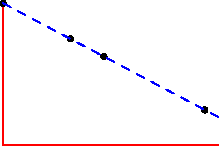
\includegraphics{reg-rsq1}
		&
		\includegraphics{reg-rsq2}
		&
		\includegraphics{reg-rsq3}
		&
		\includegraphics{reg-rsq4}
		\\
		Perfect model $R^2=1$
		&
		Useless model $R^2=0$
		&
		Good model $R^2=0.97$
		&
		Poor model $R^2=0.22$
	\end{tabular}
\end{center}


\boldinline{Efficient computation of $R^2$}

If you want to compute by hand, our current process is lengthy and awkward. To obtain a more efficient alternative we first consider an alternative expression for the variance of any collection of data:
\[
	\Var x=\frac 1n\sum(x_i-\cl x)^2=\frac 1n\sum x_i^2-\frac{2\cl x}n\sum x_i+\frac{\cl x}n\sum x_i =\cl{x^2}-\cl x^2
\]
Plainly $\Var x\ge 0$ with equality if and only if all data values $x_i$ are equal. The alternative expression $\cl{x^2}-\cl x^2$ justifies the uniqueness of the regression line in Definition \ref{defn:regdef} and Theorem \ref{thm:linreg}.

\goodbreak

Now expand the variance of the predicted outputs:
\[
	\Var\hat y=\frac 1n\sum(\hat y_i-\cl y)^2=\frac 1n\sum\bigl(mt_i+c-(m\cl t+c)\bigr)^2 =\frac{m^2}n\sum(t_i-\cl t)^2=m^2\Var t
\]
Putting these together, we obtain several equivalent expressions for the coefficient of determination:\phantomsection\label{pg:rsqalt}
\[
	R^2 =\frac{\Var\hat y}{\Var y} 
	=m^2\frac{\Var t}{\Var y} 
	=m^2\frac{\cl{t^2}-\cl t^2}{\cl{y^2}-\cl y^2}
	=\frac{(\cl{ty}-\cl t\cl y)^2}{(\cl{t^2}-\cl t^2)(\cl{y^2}-\cl y^2)}
%=1-\frac{\sum e_i^2}{n\Var y} %=\frac{\Cov(y,t)}{\sqrt{\Var y\Var t}}
\tag{$\ast$}
\]

\begin{example}{}{finalreg}
	We do one more easy example with simple data $(t_i,y_i):(1,4),(2,1),(3,2),(4,0)$.\par
	\begin{minipage}[t]{0.55\linewidth}\vspace{-10pt}
		\begin{gather*}\renewcommand{\arraystretch}{1.3}
			\begin{array}{|c|cccc|c|}
				\hline
				\multicolumn{5}{|c|}{\text{data}}&\text{average}\\\hline
				t_i&1&2&3&4&\cl t=\frac{10}4\\\hline
				y_i&4&1&2&0&\cl y=\frac 74\\\hline
				t_i^2&1&4&9&16&\cl{t^2}=\frac{15}2\\\hline
				y_i^2&16&1&4&0&\cl{y^2}=\frac{21}4\\\hline
				t_iy_i&4&2&6&0&\cl{ty}=3\\\hline
			\end{array}\\[5pt]
			m=\frac{\cl{ty}-\cl t\cl y}{\cl{t^2}-\cl t^2} =\frac{3-\frac{70}{4^2}}{\frac{15}2-\frac{100}{4^2}} =-\frac{11}{10}=-1.1\\
			c=\cl y-m\cl t=\frac{7}4+\frac{11\cdot 10}{10\cdot 4}=\frac 92 =4.5
		\end{gather*}
\end{minipage}
\hfill
\begin{minipage}[t]{0.44\linewidth}\vspace{0pt}
	\flushright\includegraphics{reg-line5}
\end{minipage}\medbreak
The regression line is $\hat y=-\frac{11}{10}t+\frac 92=-1.1t+4.5$, and the coefficient of determination is
\[
	R^2=m^2\frac{\cl{t^2}-\cl t^2}{\cl{y^2}-\cl y^2} =\frac{121}{100}\cdot \frac{\frac{15}2-\frac{100}{4^2}}{\frac{21}4-\frac{49}{4^2}}= \frac{121}{100}\cdot \frac{20}{35} =\frac{121}{175} =69.1\%
\]
The \textcolor{Green}{minimized square error} is also easily computed:
\[
	\sum e_i^2=\sum(\hat y_i-y_i)^2=(3.4-4)^2+(2.3-1)^2+(1.2-2)^2+(0.1-0)^2=2.7
\] 
\end{example}


\boldinline{Reversion to the Mean \& Correlation}

By ($\ast$), the regression model may be re-written in terms of the standard-deviation and $R^2$: 
\[
	\hat y(t)=mt+c=\cl y+m(t-\cl t) =\cl y+\textcolor{red}{\sqrt{R^2}}\frac{\sigma_y}{\sigma_t}(t-\cl t) \implies \hat y(\cl t+\lambda\sigma_t)=\cl y+\lambda\textcolor{red}{\sqrt{R^2}}\sigma_y
\]

\begin{defn}{}{}
	The \emph{correlation coefficient} is the value $r:=\pm\sqrt{R^2}$ (sign equal to that of $m$).
\end{defn}

An input $\lambda$ standard-deviations above the mean ($t=\cl t+\lambda\sigma_t$) results in a prediction $\lambda r$ standard-deviations above the mean ($\hat y=\cl y+\lambda r\sigma_y$). Unless the data is perfectly linear, we have $R^2<1$; relative to the `neutral' measure given by the standard-deviation a prediction $\hat y(t)$ is closer to the mean than the input $t$
\[
	\frac{\nm{\hat y(t)-\cl y}}{\sigma_y} =r\frac{\nm{\hat t-\cl t}}{\sigma_t}
	<\frac{\nm{\hat t-\cl t}}{\sigma_t}
\]




\goodbreak


\begin{example*}{\ref{ex:finalreg}, cont}{}
	We compute the details. The correlation coefficient is $r=-\sqrt{R^2}\approx -0.832$; we say that the data is \emph{negatively correlated,} since the output $y$ seems to \emph{decrease} as $t$ increases. The standard deviations may be read off from the table:
	\[
		\sigma_t=\sqrt{\Var t}=\sqrt{\cl{t^2}-\cl t^2}=\frac{\sqrt 5}2\approx 1.118,\qquad \sigma_y=\sqrt{\Var y}=\sqrt{\cl{y^2}-\cl y^2}=\frac{\sqrt{35}}4\approx 1.479
	\]
	The predictor may therefore be written (approximately)
	\[
		\hat y(\cl t+\lambda\sigma_t)=\hat y(2.5+1.12\lambda) =\cl y+\lambda r\sigma_y =1.75-1.23\lambda
	\]
	As a sanity check,
	\[
		\hat y(2.5+1.12)=\hat y(3.62)=-1.1\times -3.98+4.5=0.52 =1.75-1.23
	\]
\end{example*}


\boldinline{Weaknesses of Linear Regression}

There are two obvious issues:
\begin{itemize}
  \item Outliers massively influence the regression line. Dealing with this problem is complicated and there are a variety of approaches that can be used. It is important to remember that any approach to modelling, including our regression model, requires some \emph{subjective choice.}
  \item If the data is not very linear then the regression model will produce a weak predictor. There are several ways around this as we'll see in the remaining sections: higher-degree polynomial regression can be performed, and data sometimes becomes more linear after some manipulation, say by an exponential or logarithmic function.
\end{itemize}


\begin{exercises}{}{}
	\exstart Suppose $(z_i)=(2,4,10,8)$ is \emph{double} the data set in Example \ref{ex:vareasy}. Find $\cl z,\Var z$ and $\sigma_z$. Why are you not surprised?
	
	\begin{enumerate}\setcounter{enumi}{1}
	  \item Use a spreadsheet to find $R^2$ for the predictor in Exercise \ref*{sec:reg1}.\ref{exs:kidsheights}. How confident do you feel in your prediction?
	  
	  
	  \item Find the standard deviations and correlation coefficients for the data in Examples \ref{ex:reg1} and \ref{ex:reg2}.
	  
	  
	  \item The adult heights of men and women in a given population satisfy the following:
	  \begin{quote}
	  	Men:\lstsp average 69.5\,in, \ $\sigma=3.2$\,in.\qquad
	  	Women:\lstsp average 63.7\,in, \ $\sigma=2.5$\,in.
	  \end{quote}
	  The height of a father and his adult daughter have correlation coefficient $0.35$. If a father's height is 72\,in (mother's height unknown), how tall do you expect their daughter to be?
	
	  
	  \item Suppose $R^2$ is the coefficient of determination for a linear regression model $\hat y=mt+c$. Use one of the alternative expressions for $R^2$ (page \pageref{pg:rsqalt}) to find the coefficient of determination for the reversed predictor $\hat t(y)$? Are you surprised?
	  	  
	  
	  \item\label{exs:Rsqalt} Suppose that a data set $\{(t_i,y_i)\}_{1\le i\le n}$ has at least two distinct $t$- and $y$-values (some $t_i\neq t_j$, etc.), that it has regression line $\hat y=mt+c$ and coefficient of determination $R^2$.
	  \begin{enumerate}
	    \item Show that $R^2=0\Longleftrightarrow m=0$.
	    \item (Hard)\lstsp Prove that the sum of squared errors equals $S=\sum_{i=1}^ne_i^2 =n(\Var y-\Var\hat y)$.
	    \item Obtain the alternative expression $R^2=1-\frac S{n\Var y}$. Hence conclude that $R^2\le 1$, with equality if and only if the original data set is perfectly linear.
		\end{enumerate}	
	\end{enumerate}

\end{exercises}

\clearpage



\subsection{Matrix Multiplication \& Polynomial Regression}

In this section we consider how to find a best-fitting least-squares polynomial for given data. To see how to do this, it helps to rephrase the linear approach using matrices.\footnote{Matrix computations are non-examinable. The purpose of this section is to be see how the regression may easily be automated and generalized by computer and to understand a little of how a spreadsheet calculates best-fitting curves of different types.}
\bigskip

\iffalse
This is a very quick primer on how to multiply matrices. It is very easy if you are comfortable with the dot product! As an application, we obtain a useful way to think about the system of equations involved in linear regression which extends easily to polynomial regression. 
\begin{itemize}
  \item An $m\times n$ matrix is an array of $mn$ numbers with $m$ rows and $n$ columns. Here, for example, is a $3\times 4$ matrix,
  \[\begin{pmatrix}
  3&2&0&0\\
  -2&\frac 12&-1&0\\
  0&4&1&-1
  \end{pmatrix}\]
  \item Suppose $A$ is $m\times n$ and $B$ is $n\times r$. If $a_{ij}$ is the entry in the $i\th$ row, $j\th$ column of $A$ (and similarly for $B$), then the product $AB$ is the $m\times r$ matrix with $ik\th$ entry
  \[(AB)_{ik}=\sum_{j=1}^na_{ij}b_{jk} =a_{i1}b_{1k}+a_{i2}b_{2k}+\cdots +a_{in}b_{nk}\]
  Equivalently, if we write $A=\sthreevec{\va_1^T}{\vdots}{\va_n^T}$ in terms of its $n$ \emph{rows,} and $B=(\vb_1\ \ldots\ \vb_n)$ in terms of its $n$ \emph{columns,} then the $i\th$ row $j\th$ column of $AB$ is the dot product $\va_i\cdot \vb_j$. This is often said as ``multiply along the row and down the column.'' For example
  \[\begin{pmatrix}
  \textcolor{red}{3}&\textcolor{red}{2}&\textcolor{red}{0}\\
  -2&1&3
  \end{pmatrix}\begin{pmatrix}
  1&\textcolor{red}{2}&2&0\\
  -2&\textcolor{red}{-1}&3&1\\
  0&\textcolor{red}{5}&-1&1
  \end{pmatrix}
  =\begin{pmatrix}
  -1&\textcolor{red}{4}&12&2\\
  -4&12&-4&4
  \end{pmatrix}\]
  where the 1\st\ row 2\nd\ column of the product was computed via
  \[\begin{pmatrix}
  \textcolor{red}{3}&\textcolor{red}{2}&\textcolor{red}{0}
  \end{pmatrix}\begin{pmatrix}
  \textcolor{red}{2}\\
  \textcolor{red}{-1}\\
  \textcolor{red}{5}
  \end{pmatrix} =3\cdot 2+2(-1)+0\cdot 5 =\,\textcolor{red}{4}\]
  \item The $m\times m$ \emph{identity} matrix has all of its entries zero, \emph{except} down the main diagonal, all of whose entries are 1. For instance, the $3\times 3$ identity matrix is
  \[I=\begin{pmatrix}
  1&0&0\\0&1&0\\0&0&1
  \end{pmatrix}\]
  The identity behaves very like the number 1: for any matrix $A$, we have $IA=AI=A$.
  \item A square matrix $A$ has an \emph{inverse} $A^{-1}$ if
  $AA^{-1}=A^{-1}A=I$.
  For $2\times 2$ matrices there is an explicit formula, provided $ad-bc\neq 0$,
  \[\begin{pmatrix}
  a&b\\c&d
  \end{pmatrix}^{-1}
  =\frac 1{ad-bc}\begin{pmatrix}
  d&-b\\-c&a
  \end{pmatrix}
  \]
  Explicit formulas can be found for larger matrices, though they aren't practically useful. We won't explicitly invert anything beyond $2\times 2$. Just know that computers are expert at this!
\end{itemize}
\fi

We start by observing that the system of equations in Theorem \ref{thm:linreg} can be written in as a $2\times 2$ matrix problem. For a data set with $n$ pairs, the coefficients $m,c$ satisfy
\[
	\begin{pmatrix}
		\sum t_i^2&\sum t_i\\
		\sum t_i&n
	\end{pmatrix}
	\twovec mc=\twovec{\sum t_iy_i}{\sum y_i}
\]
This is nice because we can decompose the square matrix on the left as the product of a simple $2\times n$ matrix and its transpose (switch the rows and columns);
\[
	\begin{pmatrix}
		\sum t_i^2&\sum t_i\\
		\sum t_i&n
	\end{pmatrix}
	=
	\begin{pmatrix}
		t_1&t_2&\cdots&t_n\\
		1&1&\cdots&1
	\end{pmatrix}
	\begin{pmatrix}
		t_1&1\\
		t_2&1\\
		\vdots&\vdots\\
		t_n&1
	\end{pmatrix}
	=:P^TP
\]
We can also view the right side as the product of $P^T$ and the column vector of output values $y_i$:
\[
	\twovec{\sum t_iy_i}{\sum y_i}=
	\begin{pmatrix}
		t_1&t_2&\cdots&t_n\\
		1&1&\cdots&1
	\end{pmatrix}
	\threevec{y_1}{\vdots}{y_n}=:P^T\vy
\]
A little theory tells us that if \emph{at least two} of the $t_i$ are distinct, then the $2\times 2$ matrix $P^TP$ is invertible;\footnote{%
For those who've studied linear algebra, $P$ and $P^TP$ have the same null space and thus rank, since
	\[
		P\vx=\V0\implies P^TP\vx=\V0\quad\text{and}\quad P^TP\vx=\V0\implies \vx^TP^TP\vx=\V0\implies \Nm{P\vx}=\V0\implies P\vx=\V0
	\]
	For linear regression, having at least two distinct $t_i$ values means $\Rank P=2$, whence $P^TP$ is invertible.
}
there is a \emph{unique} regression line whose coefficients may be found by taking the matrix inverse
\[
	\twovec mc=(P^TP)^{-1}P^T\vy \implies \hat y=mt+c=(t\ \ 1)\twovec mc=(t\ \ 1)(P^TP)^{-1}P^T\vy
\]
We can also easily compute the vector of predicted values $\hat y_i=\hat y(t_i)$:
\[
	\hat\vy=
	\begin{pmatrix}
		t_1&t_2&\cdots&t_n\\
		1&1&\cdots&1
	\end{pmatrix}
	\twovec mc=P(P^TP)^{-1}P^T\vy
\]
and the squared error $\sum e_i^2=\sum\nm{\hat y_i-y_i}^2=\Nm{\hat\vy-\vy}^2$, which leads to an alternative expression for the coefficient of determination
\[
	R^2=\frac{\Nm{\hat\vy}^2-n\cl y^2}{\Nm\vy^2-n\cl y^2}
\]
where $\Nm\vy$ is the \emph{length} of a vector.

\goodbreak


\begin{examples}{}{}
	\exstart We revisit the Example \ref{ex:finalreg} in this language.
	\[
		P=
		\begin{pmatrix}
			t_1&1\\
			t_2&1\\
			\vdots&\vdots\\
			t_n&1
		\end{pmatrix}
		=
		\begin{pmatrix}
			1&1\\
			2&1\\
			3&1\\
			4&1
		\end{pmatrix}
		\implies P^TP=
		\begin{pmatrix}
			1&2&3&4\\
			1&1&1&1
		\end{pmatrix}
		\begin{pmatrix}
			1&1\\
			2&1\\
			3&1\\
			4&1
		\end{pmatrix}
		=
		\begin{pmatrix}
			30&10\\
			10&4
		\end{pmatrix}
	\]
	from which
	\begin{align*}
		\twovec mc&=(P^TP)^{-1}P^T\vy =
		\begin{pmatrix}
			30&10\\
			10&4
		\end{pmatrix}^{-1}
		\begin{pmatrix}
			1&2&3&4\\
			1&1&1&1
		\end{pmatrix}
		\smash[t]{\fourvec 4120}\\
		&=\frac 1{30\cdot 4-10^2}
		\begin{pmatrix}
			4&-10\\
			-10&30
		\end{pmatrix}
		\twovec{12}{7} =\frac 1{20}\twovec{48-70}{-120+210}=\frac 1{10}\twovec{-11}{45}
	\end{align*}
	The prediction vector given inputs $t_i$ is therefore
	\[
		\hat\vy=P\twovec mc=\frac 1{10}
		\begin{pmatrix}
			1&2&3&4\\
			1&1&1&1
		\end{pmatrix}
		\twovec{-11}{45} =\frac 1{10}\fourvec{34}{23}{12}{1}
	\]
	from which the coefficient of determination is, as before
	\[
		R^2=\frac{\Nm{\hat\vy}^2-4\cl y^2}{\Nm\vy^2-4\cl y^2} =\frac{\frac 1{100}(34^2+23^2+12^2+1^2)-4\cdot\frac{7^2}{4^2}}{(4^2+1^1+2^2+0^2)-4\cdot\frac{7^2}{4^2}} =\frac{121}{175}
	\]
	\begin{enumerate}\setcounter{enumi}{1}
	  \begin{minipage}[t]{0.65\linewidth}\vspace{0pt}
		  \item Given the data set $\{(3,1),(3,5),(3,6)\}$, we have $P=
		  \begin{smatrix}
		   3&1\\
		   3&1\\
		   3&1
		  \end{smatrix}$ and $P^TP=
		  \begin{smatrix}
		   27&9\\9&3
		  \end{smatrix}$ 
		  which isn't invertible: $27\cdot 3-9\cdot 9=0$. The linear regression method doesn't work!\smallbreak
		  It is easy to understand this from the picture. Since the three data points are vertically aligned, any \textcolor{blue}{line} minimizing the sum of the squared errors must pass through the \textcolor{Green}{average} $(3,4)$, though it could have \emph{any} slope!\par
		  This illustrates our fundamental assumption: linear regression requires at least two distinct $t$-values.
		\end{minipage}
		\hfill
		\begin{minipage}[t]{0.34\linewidth}\vspace{0pt}
		  \flushright\includegraphics{reg-line6}
	  \end{minipage}
	\end{enumerate}
\end{examples}

It is unnecessary ever to use the matrix approach for linear regression, though the method has significant advantages.
\begin{itemize}\itemsep2pt
  \item Computers store and manipulate data in matrix format, so this method is computer-ready.
  \item Suppose you repeat an experiment several times, taking measurements $y_i$ at times $t_i$. Since $P$ depends only on the $t$-data, you need only compute the matrix $(P^TP)^{-1}P^T$ \emph{once}, making computation of the regression line for repeat experiments very efficient. 
  \item The method generalizes (easily for computers!) to polynomial regression\ldots
\end{itemize}


\goodbreak


\boldsubsubsection{Polynomial Regression}

The pattern is almost identical when we use matrices; you just need to make the matrix $P$ a little larger\ldots We work through the approach for a quadratic approximation.\smallbreak

Suppose we have a data set $\{(t_i,y_i):1\le i\le n\}$ and that we desire a quadratic polynomial predictor $\hat y=at^2+bt+c$ which minimizes the sum of the squared vertical errors
\[
	S(a,b,c)=\sum_{i=1}^n e_i^2=\sum_{i=1}^n(at_i^2+bt_i+c-y_i)^2
\]
This might look terrifying, but can be attacked exactly as before using differentiation: to minimize $S$, we need the derivatives of $S$ with respect to the coefficients $a,b,c$ to be zero.
\begin{gather*}
	\def\arraystretch{1.9}
	\left\{
	\begin{array}{@{}lll}
		\displaystyle\partials[S]{a}=2\sum at_i^4+bt_i^3+ct_i^2-t_i^2y_i=0\\
		\displaystyle\partials[S]{b}=2\sum at_i^3+bt_i^2+ct_i-t_iy_i=0\\
		\displaystyle\partials[S]{c}=2\sum at_i^2+bt_i+c-y_i=0
	\end{array}
	\right.
	\iff
	\left\{
	\begin{array}{@{}lll}
		\displaystyle a\sum t_i^4+b\sum t_i^3+c\sum t_i^2=\sum t_i^2y_i\\
		\displaystyle a\sum t_i^3+b\sum t_i^2+c\sum t_i=\sum t_iy_i\\
		\displaystyle a\sum t_i^2+b\sum t_i+cn=\sum y_i
	\end{array}
	\right.
\end{gather*}
As a system of equations for $a,b,c$ this looks fairly nasty, but by rephrasing in terms of matrices, we see that it is exactly the same problem as before!
\[
	\begin{pmatrix}
		\sum t_i^4 & \sum t_i^3 & \sum t_i^2\\
		\sum t_i^3 & \sum t_i^2 & \sum t_i\\
		\sum t_i^2 & \sum t_i & cn
	\end{pmatrix}
	\threevec abc=\threevec{\sum t_i^2y_i}{\sum t_iy_i}{\sum y_i}
\]
corresponds to
\[
	P^TP\threevec abc=P^T\vy
	\quad\text{where}\quad
	P=
	\begin{pmatrix}
		t_1^2&t_1&1\\
		\vdots&\vdots&\vdots\\
		t_n^2&t_n&1
	\end{pmatrix}
	\quad \text{and}
	\quad\vy=\threevec{y_1}{\vdots}{y_n}
\]
The only change is that $P$ is now an $n\times 3$ matrix so that $P^TP$ is $3\times 3$. Analogous to the linear situation, provided at least three of the $t_i$ are distinct, the matrix $P^TP$ is invertible and there is a unique least-squares quadratic minimizer
\[
	\hat y=at^2+bt+c=\bigl(t^2\ \ t\ \ 1\bigr)\threevec a bc =\bigl(t^2\ \ t\ \ 1\bigr)(P^TP)^{-1}P^T\vy
\]
The predictions $\hat y_i=\hat y(t_i)$ therefore form a vector $\hat\vy=P\sthreevec ab c=P(P^TP)^{-1}P^T\vy$, and the coefficient of determination may be computed as before.
\[
	R^2=\frac{\Nm{\hat\vy}^2-n\cl y^2}{\Nm\vy^2-n\cl y^2}
\]
\smallbreak
The method generalizes in the obvious way: if you want a cubic minimizer, give $P$ an extra column of \emph{cubed} $t_i$-terms! This would be hard work by hand, but is standard fodder for computers: this isn't a linear algebra class, so don't try to invert a $3\times 3$ matrix!


\goodbreak


\begin{example}{}{}
	We are given \href{http://math.uci.edu/~ndonalds/math8/poly-ex.xlsx}{data} $\{(t_i,y_i)\}=\{(1,2),(2,5),(3,7),(4,4)\}$.
	\begin{enumerate}
	  \item For the best-fitting linear model, we use the same $P$ (and thus $P^TP$) from the previous example:
	  \begin{align*}
	  	\twovec mc&=(P^TP)^{-1}P^T\vy=
	  	\begin{pmatrix}
				30&10\\
				10&4
			\end{pmatrix}^{-1}
			\!\!
			\begin{pmatrix}
				1&2&3&4\\
				1&1&1&1
			\end{pmatrix}
			\!\!\fourvec{2}{5}{7}{4} =\frac 1{10}
			\begin{pmatrix}
				2&-5\\
				-5&15
			\end{pmatrix}
			\!\!\twovec{49}{18} =\twovec{0.8}{2.5}
		\end{align*}
		which yields $\hat y(t)=0.8t+2.5$. The predicted values and coefficient of determination are then
		\[
			\hat\vy=
			\begin{pmatrix}
				1&2&3&4\\
				1&1&1&1
			\end{pmatrix}
			\twovec{0.8}{2.5}=\fourvec{3.3}{4.1}{4.9}{5.7}\qquad R^2=\frac{84.2-81}{94-81}\approx 0.2462
		\]
		The \textcolor{blue}{linear model} predicts only 24.6\% of the variance in the output; not very accurate.
		
		\item For a quadratic model; all that changes is the matrix $P$%, though the numbers are significantly less pleasant!
		\begin{gather*}
			P=
			\begin{pmatrix}
				1&1&1\\
				4&2&1\\
				9&3&1\\
				16&4&1
			\end{pmatrix}
			\implies P^TP=
			\begin{pmatrix}
				1&4&9&16\\
				1&2&3&4\\
				1&1&1&1
			\end{pmatrix}
			\begin{pmatrix}
				1&1&1\\
				4&2&1\\
				9&3&1\\
				16&4&1
			\end{pmatrix}
			=
			\begin{pmatrix}
				354&100&30\\
				100&30&10\\
				30&10&4
			\end{pmatrix}\\
			\implies \threevec abc=(P^TP)^{-1}P^T\smash[t]{\fourvec 2574}=
			\begin{pmatrix}
				354&100&30\\
				100&30&10\\
				30&10&4
			\end{pmatrix}^{-1}
			\threevec{149}{49}{18}=\threevec{-1.5}{8.3}{-5}
		\end{gather*}
		from which $\hat y=-1.5t^2+8.3t-5$. To quantify its accuracy, compute the vector of predicted values $\hat y_i=\hat y(t_i)$ and the coefficient of determination:
		\begin{gather*}
			\hat\vy=P\threevec{-1.5}{8.3}{-5}=\fourvec{1.8}{5.6}{6.4}{4.2}\qquad\qquad
			R^2=\frac{\Nm{\hat\vy}^2-4\cl y^2}{\Nm\vy^2-4\cl y^2}=\frac{93.2-81}{94-81} \approx 0.9385
		\end{gather*}\par
		
		\begin{minipage}[t]{0.58\linewidth}\vspace{-5pt}
			The \textcolor{orange}{quadratic} model is far superior to the \textcolor{blue}{linear}, explaining 94\% of the observed variance.
			
			\item We can even find a \textcolor{magenta}{cubic} model ($P$ is a $4\times 4$ matrix!)
			\[
				\hat y=\frac 1{6}(-4t^3+21t^2-17t+12)
			\]
			The cubic passes through all four data points, there is \emph{no error} and $R^2=1$.
		\end{minipage}
		\hfill
		\begin{minipage}[t]{0.4\linewidth}\vspace{-12pt}
			\flushright\includegraphics[scale=1]{reg-quad1}
		\end{minipage}
		\smallbreak
		For real-world data this is possibly \emph{less useful} than the quadratic model---it certainly takes longer to find! More importantly, likely experimental error in the $y$-data has a strong effect on the `perfect' model---we are, in effect, modelling \emph{noise.} Do you expect $y(5)$ to be closer to $\textcolor{orange}{-1}$ or $\textcolor{magenta}{-8}$?
	\end{enumerate}
\end{example}

\goodbreak


% In general, we have the following result:
% 
% \begin{thm}{Polynomial regression}{}
% Let $d$ be a positive integer and suppose $\{(t_i,y_i):1\le i\le n\}$ is a data set consisting of $n\ge d-1$ points and where \emph{at least} $d-1$ of the $t_i$ values are distinct. Then the data has a unique best-fitting least-squares polynomial of degree $d$
% \[\hat y=\sum_{k=0}^da_kt^k=a_dt^k+a_{d-1}t^{k-1}+\cdots+a_1t+a_0\]
% where the coefficients $\va$ are the unique solution to the $(d+1)\times(d+1)$ matrix problem
% \[\va=\threevec{a_d}\vdots {a_0}=(P^TP)^{-1}P^T\vy\quad\text{where}\quad P=\begin{pmatrix}
% t_1^d&t_1^{d-1}&\cdots&t_1&1\\
% \vdots&\vdots&&\vdots\\
% t_n^d&t_n^{d-1}&\cdots&t_n&1
% \end{pmatrix}\quad \text{and}
% \quad\vy=\threevec{y_1}{\vdots}{y_n}\]
% The vector of predictions $\hat y_i=\hat y(t_i)$ is $\hat\vy=P\va=P(P^TP)^{-1}\vy$, and the coefficient of determination
% \[R^2=\frac{\Nm{\hat\vy}^2-n\cl y^2}{\Nm{\vy}^2-n\cl y^2}\]
% \end{thm}

\begin{exercises}{}{}
	\exstart Recall Example \ref{ex:almostquadseq}, with the following \emph{almost} linear data set.
	\[
		\begin{array}{c|cccccc}
			x&0&2&4&6&8&10\\\hline
			y&3&23&41&59&77&93
		\end{array}
	\]
	Find the best-fitting straight line for the data, then use a spreadsheet to find the best-fitting quadratic. Is the extra effort worth it? 
	
	\begin{enumerate}\setcounter{enumi}{1}
	  \item You are given the following data consisting of measurements from an experiment recorded at times $t_i$ seconds.
	  \[
	  	\begin{array}{c|cccccccccc}
	  		t_i&1&2&3&4&5&6&7&8&9&10\\\hline
	  		y_i&7&5&3&2&3&5&6&9&8&12
	  	\end{array}
	  \]
	  \begin{enumerate}
	    \item Given the values
	  	\[
	  		\sum t_i=55,\quad \sum t_i^2=385,\quad \sum y_i=60,\quad \sum t_iy_i=385
	  	\]
	  	find the best-fitting least-squares linear model for this data, and use it to predict $\hat y(13)$.
	    
	    \item Find the best-fitting quadratic model for the data: feel free to use a spreadsheet!
	    
	    \item The graphs below show the best-fitting least-squares linear, quadratic, cubic, quartic, and ninth-degree models and their coefficients of determination.
	    \begin{center}
	    	\begin{tabular}[t]{@{}c@{\quad}c@{\quad}c@{}}
	    		\includegraphics{midterm-reg1}
					&
	    		\includegraphics{midterm-reg2}
	    		&
	    		\includegraphics{midterm-reg3}
	    		\\
	    		\includegraphics{midterm-reg4}
	    		&
	    		\includegraphics{midterm-reg9}
	    		&
	    		\begin{tabular}[b]{c|c}
		    		Degree&$R^2$\\\hline
		    		1&0.4264\\
		    		2&0.8830\\
		    		3&0.9319\\
		    		4&0.9336\\
		    		\vdots&\vdots\\
		    		9&1\\
		    		\multicolumn{2}{c}{}
	    		\end{tabular}
	    	\end{tabular}
	    \end{center}
	
	    Which of these models would \emph{you} choose for this data and why? What considerations would you take into account?  
		\end{enumerate}
	\end{enumerate}
\end{exercises}


\clearpage


\subsection{Exponential \& Power Regression Models}

If you suspect that your data would be better modelled by a non-polynomial function, there are several things you can try.\medbreak

Minimizing the sum of squared-errors might be very difficult for non-polynomial functions because there is likely no simple tie-in with linear equations/algebra. Attempting this is likely to result in a horrible \emph{non-linear} system for your coefficients which is difficult to analyze either theoretically or using a computer.\footnote{%
	As an example of how horrific this is, suppose you want to minimize the sum of square-errors for data $(t_i,y_i)$ using an exponential model $\hat y(t)=ae^{kt}$. The coefficients of our model, $a,k$ should minimize
	\[
		S(a,k)=\sum_{i=1}^n\bigl(ae^{kt_i}-y_i\bigr)^2
	\]
	Differentiating this with respect to $a,k$ and setting equal to zero results in
	\[
		\begin{cases}
			\partials[S]{a}=2\sum e^{kt_i}\bigl(ae^{kt_i}-y_i\bigr)=0 \\
			\partials[S]{k}=2a\sum t_ie^{kt_i}\bigl(ae^{kt_i}-y_i\bigr)=0
		\end{cases}
		\implies  \bigl(\sum y_ie^{kt_i}\bigr)\bigl(\sum t_ie^{2kt_i}\bigr) =\bigl(\sum e^{2kt_i}\bigr)\bigl(\sum t_iy_ie^{kt_i}\bigr)
	\]
	where we substituted for $a$ to obtain the last equation. Remember that this is an equation for $k$; if you think you can solve this easily, think again!
}

\boldinline{Log Plots}

The most common approach when trying to fit an exponential model $\hat y=e^{mt+c}$ to data is to use a log plot: taking logarithms of both sides results in
\[
	\ln\hat y=mt+c
\]
If we take $\hat Y:=\ln\hat y$ as a new variable, the model is now a \emph{straight-line}! The idea is then to use linear regression to find the coefficients $m,\ln a$.

\begin{example*}{\ref{ex:poprabbits}, cont}{}
	Recall our earlier rabbit-population $P(t)$, repeated in the table below. We previously considered modelling this with an exponential function for two reasons:\par
	\begin{minipage}[t]{0.55\linewidth}\vspace{-6pt}
		\begin{enumerate}\itemsep0pt
		  \item We were told it was population data!
		  \item The \emph{$t$-differences} are constant $(2)$, while the \emph{$P$-ratios} are approximately so ($\approx 1.41$).
		\end{enumerate}
	\end{minipage}
	\hfill
	\begin{minipage}[t]{0.44\linewidth}\vspace{0pt}
		\flushright $\begin{array}{c|cccccc}
			t_i&0&2&4&6&8&10\\\hline
			P_i&5&7&10&14&19&28\\\hline\hline
			\ln P_i&1.61&1.95&2.30&2.64&2.94&3.33
		\end{array}$
		\end{minipage}\medbreak
		After constructing a log-plot, the relationship is much clearer:
		\begin{center}
			\includegraphics{rabbits3}
			\qquad\qquad
			\includegraphics{rabbits4}
		\end{center}
		Since the relationship between $t$ and $\ln P$ appears linear, we perform a linear regression calculation to find the best-fitting least-squares line for the $(t_i,\ln P_i)$ data.\par
		
		\begin{minipage}[t]{0.64\linewidth}\vspace{0pt}
			Everything necessary comes from extending the table.
			\begin{gather*}\def\arraystretch{1.2}
				\begin{array}{c|cccccc|c}
					\multicolumn{7}{c|}{\text{Data}}&\text{average}\\\hline\hline
					t_i&0&2&4&6&8&10&5\\\hline
					P_i&5&7&10&14&19&28&13.83\\\hline\hline
					\ln P_i&1.61&1.95&2.30&2.64&2.94&3.33&2.46\\\hline
					t_i^2&0&4&16&36&64&100&36.67\\\hline
					t_i\ln P_i&0&3.89&9.21&15.83&23.56&33.32&14.30
				\end{array}\\[5pt]
				m=\frac{\cl{t\ln P}-\cl t\cdot\cl{\ln P}}{\cl{t^2}-\cl t^2}=\frac{14.30-5\cdot 2.46}{36.67-5^2} =0.171\\[2pt]
				c=\cl{\ln P}-m\cl t=3.46-0.171\cdot 5=1.609
			\end{gather*}
			which yields the exponential model
			\[
				\hat P(t)=e^{0.171t+1.609}=4.998(1.186)^t
			\]
		\end{minipage}
		\hfill
		\begin{minipage}[t]{0.35\linewidth}\vspace{0pt}
			\flushright\includegraphics{rabbits5}\\
			\includegraphics{rabbits6}
	\end{minipage}\medbreak
	
	This is very close to the model ($5(1.188)^t$) we obtained previously by pure guesswork. The approximate doubling time $T$ for the population satisfies
	\[
		e^{mT}=2\implies T=\frac{\ln 2}{m}=4.06\ \text{months}
	\]
\end{example*}

When using the log plot method, interpreting errors and the goodness of fit of a model is a little more difficult. Typically one computes the coefficient of determination $R^2$ of the \emph{underlying linear model}: in our example,\footnote{This needs more decimal places of accuracy for the log-values than what's in our table!}
\[
	R^2=m^2\frac{\Var t}{\Var\ln P}=99.3\%
\]
\begin{minipage}[t]{0.6\linewidth}\vspace{0pt}
	It is important to appreciate that the log plot method does not treat all errors equally: taking logarithms tends to reduce error by a greater amount when the output  $y$ is large. This should be clear from the picture, and more formally by the mean value theorem: if $y_1<y_2$, then there is some $\xi\in(y_1,y_2)$ for which 
	\[
		\ln y_1-\ln y_2<\frac 1{\xi}(y_1-y_2)
	\]
\end{minipage}
\hfill
\begin{minipage}[t]{0.39\linewidth}\vspace{0pt}
	\flushright\includegraphics{logerror}
\end{minipage}
\medbreak

The log plot approach therefore places a higher emphasis on accurately matching data when the output $y$ is \emph{small.} This isn't such a bad thing, since our intuitive view of error depends on the size of the data. For instance, you might be very annoyed to discover that you've misplaced a \$100 bill, but if you've just bought a house for \$1 million, a \$100 mistake in escrow is unlikely to concern you very much! Exponential data can more easily vary over large orders of magnitude than linear or quadratic data. 

\goodbreak

\boldinline{Log-Log Plots} 

If you suspect a \emph{power function model} $\hat y=at^m$, then taking logarithms
\[
	\ln\hat y=m\ln t+\ln a
\]
results in a linear relationship between $\ln y$ and $\ln t$. As before, we can apply a linear regression approach to find a mode; the goodness of fit is again described by the coefficient of determination of the underlying model. 


\begin{exercises}{}{}
	\exstart You suspect a logarithmic model for a data set. Describe how you would approach finding a model in the context of this section.
	
	\begin{enumerate}\setcounter{enumi}{1}
	  \item The table shows the average weight and length of a fish species measured at different ages.\par
		\begin{minipage}[t]{0.45\linewidth}\vspace{0pt}
			\centering
			\begin{tabular}{c|c|c}
				Age (years)&Length(cm)& Weight (g)\\\hline\hline
				1 & 5.2 & 2\\
				2 & 8.5 & 8\\
				3 & 11.5 & 21\\
				4 & 14.3 & 38\\
				5 & 16.8 & 69\\
				6 & 19.2 & 117\\
				7 & 21.3 & 148\\
				8 & 23.3 & 190\\
				9 & 25.0 & 264\\
				10 & 26.7 & 293\\
				11 & 28.2 & 318\\
				12 & 29.6 & 371\\
				13 & 30.8 & 455\\
				14 & 32.0 & 504\\
				15 & 33.0 & 518\\
				16 & 34.0 & 537\\
				17 & 34.9 & 651\\
				18 & 36.4 & 719\\
				18 & 37.1 & 726\\
				20 & 37.7 & 810
			\end{tabular}
		\end{minipage}
		\hfill
		\begin{minipage}[t]{0.54\linewidth}\vspace{0pt}
			\hfill\includegraphics[scale=0.95]{fishexp}
			\vspace{-5pt}
			\begin{enumerate}
		  	\item Do you think an exponential model is a good fit for this data? Take logarithms of the weight values and use a \href{http://math.uci.edu/~ndonalds/math8/fishdata.xlsx}{spreadsheet} to obtain a model $\hat w(\ell)=ae^{m\ell}$ where $w,\ell$ are the weight and length respectively.
		  	\item What happens if you try a log-log plot? Given what we're measuring, why do you expect a power model to be mode accurate?
			\end{enumerate}
		\end{minipage}
		\medbreak
	  
	  
		\begin{minipage}[t]{0.52\linewidth}\vspace{0pt}
	  	\item Population data for Long Beach CA is given.\smallbreak
	   	Using a spreadsheet or otherwise, find linear, quadratic, exponential and logarithmic regression models for this data.\par
	   	Which of these models seems to fit the data best, and which would you trust to best predict the population in 2020?\par
	   	Look up the population of Long Beach in 2020; does it confirm your suspicions? What do you think is going on?
		\end{minipage}
		\hfill
		\begin{minipage}[t]{0.45\linewidth}\vspace{0pt}
	  	\flushright\begin{tabular}{c|c|c}
			  Year&Years since 1900&Population\\\hline
			  1900&0&2,252\\
			  1910&10&17,809\\
				1920&20&55,593\\
				1930&30&142,032\\
				1940&40&164,271\\
				1950&50&250,767\\
				1960&60&334,168\\
				1970&70&358,879\\
				1980&80&361,498\\
				1990&90&429,433\\
				2000&100&461,522\\
				2010&110&462,257%\\
				%2020&120&466,742
	  	\end{tabular}
		\end{minipage}
	  
	  
	  \item In the early 1600s, Johannes Kepler used observational data to derive his \emph{laws of planetary motion,} the third of which relates the orbital period $T$ of a planet (how long it takes to go round the sun) to its (approximate) distance $r$ from the sun.
	
		\begin{minipage}[t]{0.59\linewidth}\vspace{0pt}
			\centering\begin{tabular}{c|c|c}
				Planet&$T$ (years)&$r$ (millions km)\\\hline\hline
				Mercury & 0.24 & 58\\
				Venus & 0.61 & 110\\
				Earth & 1 & 150\\
				Mars & 1.88 & 230\\
				Jupiter & 11.9 & 780\\
				Saturn & 29.5 & 1400\\
				Uranus & 84 & 2900\\
				Neptune & 165 & 4500
			\end{tabular}
		\end{minipage}
		\hfill
		\begin{minipage}[t]{0.4\linewidth}\vspace{0pt}
			\flushright\includegraphics{kepler}
		\end{minipage}\par
		The table shows the data for all the planets. Use a \href{http://math.uci.edu/~ndonalds/math8/kepler.xlsx}{spreadsheet} to analyze this data and find a model relating $T$ to $r$.\smallbreak
		Kepler did not known about Uranus and Neptune and only had relative distances for the planets. Research the correct statement of Kepler's third law and compare it with your findings.
	\end{enumerate}
\end{exercises}